% --------------------------------------
% Document Class
% --------------------------------------
\documentclass[a4paper,11pt]{article}
% --------------------------------------



% --------------------------------------
% Use Package
% --------------------------------------


%\usepackage[francais]{babel}
%\usepackage{ucs}
\usepackage[utf8]{inputenc}
\usepackage[T1]{fontenc}

\usepackage{makeidx}
\usepackage{color}
\usepackage{graphicx}
\usepackage{float}
\usepackage[hidelinks]{hyperref} 
\usepackage{geometry}
%\usepackage{lastpage}
%\usepackage{marginnote}
\usepackage{fancyhdr}
%\usepackage{titlesec}
%\usepackage{framed}
\usepackage{amsmath}
\usepackage{empheq}
\usepackage{array}
\usepackage{multicol}
\usepackage{csquotes}
%\usepackage{adjustbox}

% insert code
\usepackage{listings}

% define our color
\usepackage{xcolor}

% code color
\definecolor{ligthyellow}{RGB}{250,247,220}
\definecolor{darkblue}{RGB}{5,10,85}
\definecolor{ligthblue}{RGB}{1,147,128}
\definecolor{darkgreen}{RGB}{8,120,51}
\definecolor{darkred}{RGB}{160,0,0}

% other color
\definecolor{ivi}{RGB}{141,107,185}

\def\verticaltext#1{\rotatebox[origin=c]{90}{\x{#1}}}


\lstset{
    language=C++,
    captionpos=b,
    extendedchars=true,
    frame=lines,
    numbers=left,
    numberstyle=\tiny,
    numbersep=5pt,
    keepspaces=true,
    breaklines=true,
    showspaces=false,
    showstringspaces=false,
    breakatwhitespace=false,
    stepnumber=1,
    showtabs=false,
    tabsize=3,
    basicstyle=\small\ttfamily,
    backgroundcolor=\color{ligthyellow},
    keywordstyle=\color{ligthblue},
    morekeywords={include, printf, uchar},
    identifierstyle=\color{darkblue},
    commentstyle=\color{darkgreen},
    stringstyle=\color{darkred},
}


% --------------------------------------



% --------------------------------------
% Page setting
% --------------------------------------
%\pagestyle{empty}
\setlength{\headheight}{15pt}

\setcounter{secnumdepth}{3}
\setcounter{tocdepth}{2}

\makeatletter
\@addtoreset{chapter}{part}
\makeatother 

\hypersetup{         % parametrage des hyperliens
  colorlinks=true,      % colorise les liens
  breaklinks=true,      % permet les retours à la ligne pour les liens trop longs
  urlcolor= blue,       % couleur des hyperliens
  linkcolor= black,     % couleur des liens internes aux documents (index, figures, tableaux, equations,...)
  citecolor= green      % couleur des liens vers les references bibliographiques
}

% --------------------------------------

% --------------------------------------
% Information
% --------------------------------------
\title{
  \noindent\hrulefill \\
  \vspace{10mm} Compte-rendu TP2 VisA: Mise en correspondance stéréoscopique
}

\author{Gaëtan DEFLANDRE}
% --------------------------------------

\definecolor{myColor}{rgb}{0.5, 0.1, 0.75}

% --------------------------------------
% Begin content
% --------------------------------------
\begin{document}


\maketitle

\noindent\hrulefill \\


\section{Introduction}
Il existe plusieurs techniques de reconstruction 3D, la stéréovision fait partie de ces techniques.
La stéréoscopie consiste à avoir deux projections perspectives donnant une géométrie épipolaire. 
Avec ces deux images et les propriétés de la géométrie épipolaire, il est possible d'effectuer une 
mise en correspondance stéréoscopique, qui est faite dans ce TP. Cette mise en correspondance nous 
permet de retrouver la profondeur.\\

\newpage

\section{Calcul de la matrice fondamentale}

En stéréovision les deux projections nous donnent deux images que nous appelons image de gauche et 
image de droite. Il existe une matrice que l'on nomme matrice fondamentale, elle caractérise la 
géométrie épipolaire liée aux deux projections. Il est nécessaire de calculer cette matrice pour 
effectuer la mise en correspondance des deux images.\\

\begin{figure}[H]
  \centering
  \shortstack{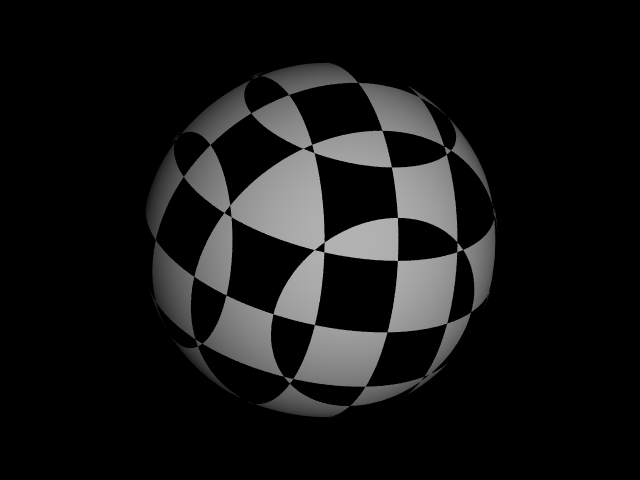
\includegraphics[width=200px]{left.png} \\ Image de gauche}
  \shortstack{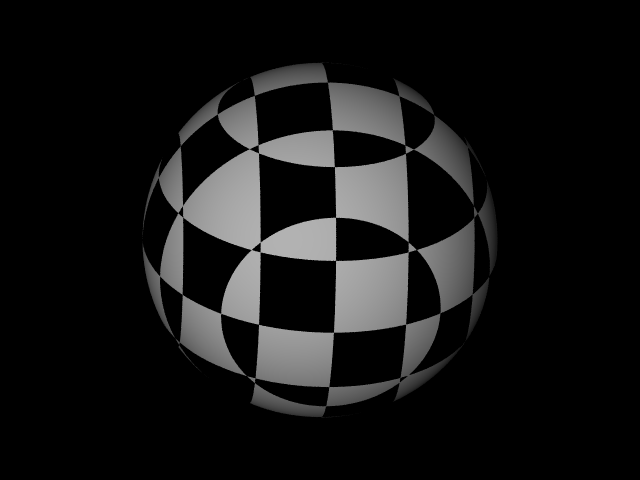
\includegraphics[width=200px]{right.png} \\ Image de droite}
\end{figure}

Formule de la matrice fondamentale:
$$
F = (P_2 O_1)^{\times} P_2 P_1^+
$$

avec le produit vectoriel:
$$
p^{\times} = 
\begin{pmatrix}
  0 && -p_z && p_y \\
  p_z && 0 && -p_x \\
  -p_y && p_x && 0 \\
\end{pmatrix}
$$

et $P^+$, la pseudo-inverse de la matrice $P$.\\

Voici les méthodes C++ pour calculer la matrice fondamentale:

\begin{lstlisting}[caption=Fonction qui calcule le produit vectoriel]
/// \brief Initialise une matrice de produit vectoriel.
///
/// @param v: vecteur colonne (3 coordonnees)
/// @return matrice de produit vectoriel
Mat iviVectorProductMatrix(const Mat& v) {

    Mat mVectorProduct = Mat::eye(3, 3, CV_64F);

    mVectorProduct.at<double>(0,0) = 0.0;
    mVectorProduct.at<double>(1,0) = -v.at<double>(Point(2,0));
    mVectorProduct.at<double>(2,0) = v.at<double>(Point(1,0));
    mVectorProduct.at<double>(0,1) = v.at<double>(Point(2,0));
    mVectorProduct.at<double>(1,1) = 0.0;
    mVectorProduct.at<double>(2,1) = -v.at<double>(Point(0,0));
    mVectorProduct.at<double>(0,2) = -v.at<double>(Point(1,0));
    mVectorProduct.at<double>(1,2) = v.at<double>(Point(0,0));
    mVectorProduct.at<double>(2,2) = 0.0;

    // Retour de la matrice
    return mVectorProduct;
}
\end{lstlisting}

\begin{lstlisting}[caption=Fonction qui calcule la matrice fondamentale]
/// \brief Initialise et calcule la matrice fondamentale.
///
/// @param mLeftIntrinsic: matrice intrinseque de la camera gauche
/// @param mLeftExtrinsic: matrice extrinseque de la camera gauche
/// @param mRightIntrinsic: matrice intrinseque de la camera droite
/// @param mRightExtrinsic: matrice extrinseque de la camera droite
/// @return matrice fondamentale
Mat iviFundamentalMatrix(const Mat& mLeftIntrinsic,
                         const Mat& mLeftExtrinsic,
                         const Mat& mRightIntrinsic,
                         const Mat& mRightExtrinsic) {

    // Doit utiliser la fonction iviVectorProductMatrix
    Mat mFundamental = Mat::eye(3, 3, CV_64F);

    Mat reduc = (Mat_<double>(3,4) <<
        1.0, 0.0, 0.0, 0.0,
        0.0, 1.0, 0.0, 0.0,
        0.0, 0.0, 1.0, 0.0
        );
    Mat p1 = mLeftIntrinsic * reduc * mLeftExtrinsic;
    Mat p2 = mRightIntrinsic * reduc * mRightExtrinsic;

    Mat iE1 = mLeftExtrinsic.inv();
    Mat o1 = iE1.col(3);

    mFundamental = iviVectorProductMatrix(p2 * o1) * p2 * p1.inv(DECOMP_SVD);

    // Retour de la matrice fondamentale
    return mFundamental;
}
\end{lstlisting}

Grâce à la matrice fondamentale, nous pouvons retrouver l'équation de la droite épipolaire 
de l'image droite associée au centre de l'image de gauche. Equation: $d_2=Fc_1$, où $F$ est 
la matrice fondamentale et $c_1$ le centre de l'image de gauche.\\

Inversement, l'équation de la droite épipolaire de l'image gauche associée au centre de l'image 
de droite est $d_1=F^Tc_2$. Il faut transposer la matrice fondamentale.\\



\section{Recherche des points homologues}

La méthode que nous utilisons pour la mise en correspondance stéréoscopique consiste en plusieurs
étapes:

\begin{itemize}
 \item Extraire les points caractéristiques des images.
 \item Calculer les droites épipolaires dans l'image de droite pour les points de l'image de 
 gauche et vise versa.
 \item Calculer les distances entre les points et les droites.
 \item Recherche les points homologues aux deux images.
\end{itemize}

\subsection{Extraction des points}

Nous retrouvons les points caractéristiques (coins) dans les deux images avec la méthode 
\textbf{Good Feature to Track} proposée par Jianbo Shi et Carlo Tomasi. Cette technique est 
très largement utilisée en vision et est implémentée sur opencv.

\begin{lstlisting}[caption=Fonction d'extraction des coins]
/// \brief Detecte les coins.
///
/// @param mImage: pointeur vers la structure image openCV
/// @param iMaxCorners: nombre maximum de coins detectes
/// @return matrice des coins
Mat iviDetectCorners(const Mat& mImage,
                     int iMaxCorners) {
    // A modifier !
    double tx = mImage.cols, ty = mImage.rows;

    vector<Point> corners = vector<Point>();

    goodFeaturesToTrack(mImage, corners, iMaxCorners, 0.01, 10);

    unsigned int nbPoint = corners.size();
    Mat mCorners = Mat(3, nbPoint, CV_64F);

    for (int i=0; i<nbPoint; i++){
        mCorners.at<double>(0,i) = corners[i].x;
        mCorners.at<double>(1,i) = corners[i].y;
        mCorners.at<double>(2,i) = 1;
    }

    //std::cout << mCorners << std::endl;

    // Retour de la matrice
    return mCorners;
}
\end{lstlisting}

\begin{figure}[H]
  \centering
  \shortstack{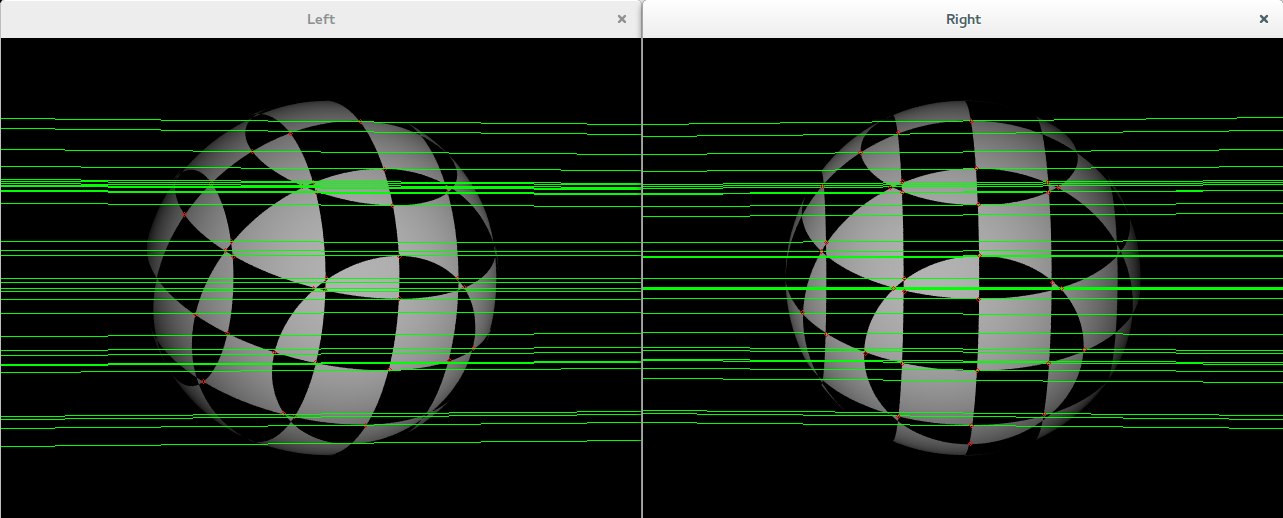
\includegraphics[width=400px]{droites_epipolaires.png} \\ Good Features et leurs droites épipolaires}
\end{figure}

\subsection{Calcul des distance}

La distance entre un point et une droite est la distance entre ce point et sa projection sur la 
droite. Nous avons l'équation de la droite $d=ax+by+c$ et les coordonnées du point $(p_x,p_y)$.
La distance est calculable avec l'équation suivante:

$$
distance = \frac{|ap_x + bp_y + c|}{\sqrt{a^2+b^2}}
$$

Dans le programme, nous conservons dans une matrice bi-dimensionnelle les résultats des distances 
de chaque point par rapport aux droites épipolaires dans l'autre image.\\



\begin{tabular}{cc}
  \  & indice des points de l'image droite \\
  \verticaltext{indice des points de l'image gauche} &
$\begin{bmatrix}
  \ldots & \ldots & \ldots \\
  \ldots & \ldots & \ldots \\
  \ldots & \ldots & \ldots \\
\end{bmatrix}
$ \\
\end{tabular}\\


\begin{lstlisting}[caption=Fontion de calcul des distances]
/// \brief Initialise et calcule la matrice des distances entres les
/// points de paires candidates a la correspondance.
///
/// @param mLeftCorners: liste des points 2D image gauche
/// @param mRightCorners: liste des points 2D image droite
/// @param mFundamental: matrice fondamentale
/// @return matrice des distances entre points des paires
Mat iviDistancesMatrix(const Mat& m2DLeftCorners,
                       const Mat& m2DRightCorners,
                       const Mat& mFundamental) {
    // A modifier !

    unsigned lenLeft = m2DLeftCorners.cols;
    unsigned lenRight = m2DRightCorners.cols;
    Mat mDistances = Mat(lenLeft, lenRight, CV_64F);

    for(unsigned i=0; i<lenLeft; i++){

        for(unsigned j=0; j<lenRight; j++){

            Mat m1 = m2DLeftCorners.col(i);
            Mat m2 = m2DRightCorners.col(j);
            Mat d2 = mFundamental * m1;
            Mat d1 = mFundamental.t() * m2;

            double dist1 = fabs(d2.at<double>(0,0)*m1.at<double>(0,0) + d2.at<double>(1,0)*m1.at<double>(1,0) + d2.at<double>(2,0))
                            / sqrt(d2.at<double>(0,0)*d2.at<double>(0,0) + d2.at<double>(1,0)*d2.at<double>(1,0));

            double dist2 = fabs(d1.at<double>(0,0)*m2.at<double>(0,0) + d1.at<double>(1,0)*m2.at<double>(1,0) + d1.at<double>(2,0))
                            / sqrt(d1.at<double>(0,0)*d1.at<double>(0,0) + d1.at<double>(1,0)*d1.at<double>(1,0));

            double dist = dist1 + dist2;

            mDistances.at<double>(i,j) = dist;
        }
    }

    // Retour de la matrice fondamentale
    return mDistances;
}
\end{lstlisting}



\section{Conclusion}



\section{Annexe}



\end{document}
